\documentclass[tikz,border=2pt]{standalone}
\usepackage{amsmath,amssymb}
\usepackage{libertinus}
\usetikzlibrary{arrows.meta,calc}

\begin{document}
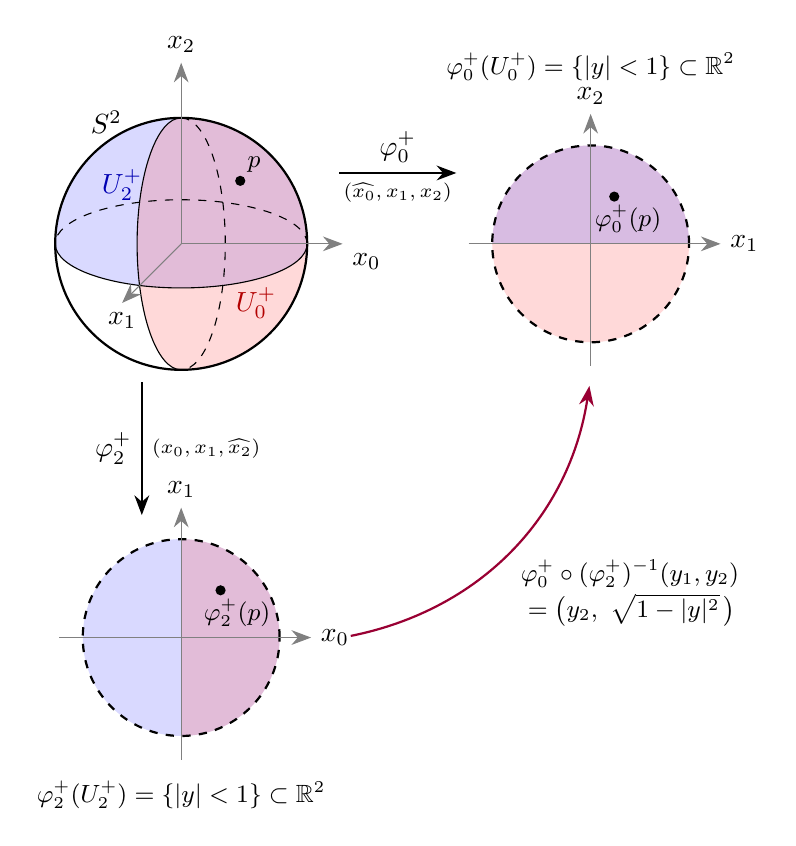
\begin{tikzpicture}[
    >={Stealth[length=2.5mm]},
    chart/.style={->,thick,shorten >=3pt,shorten <=3pt},
    U2/.style={fill=blue!60,fill opacity=0.25},
    U0/.style={fill=red!60,fill opacity=0.25},
    pt/.style={circle,fill=black,inner sep=1.3pt}
]
\def\R{1.6}   % radius of the sphere
\def\e{0.35}  % flattening of the great-circle ellipses
\def\r{1.25}  % radius of the open unit disks (chart images)

%=============================== the sphere S^2 ===============================
% U_2^+ = {x_2 > 0}: upper hemisphere (boundary: equator x_2 = 0)
\fill[U2] (-\R,0) arc[start angle=180,end angle=0,radius=\R]
          arc[start angle=0,end angle=-180,x radius=\R,y radius=\e*\R] -- cycle;
% U_0^+ = {x_0 > 0}: right hemisphere (boundary: great circle x_0 = 0)
\fill[U0] (0,-\R) arc[start angle=-90,end angle=90,radius=\R]
          arc[start angle=90,end angle=270,x radius=\e*\R,y radius=\R] -- cycle;

\draw[thick] (0,0) circle (\R);
% equator x_2 = 0
\draw[dashed] (\R,0) arc[start angle=0,end angle=180,x radius=\R,y radius=\e*\R];
\draw         (\R,0) arc[start angle=0,end angle=-180,x radius=\R,y radius=\e*\R];
% great circle x_0 = 0
\draw[dashed] (0,\R) arc[start angle=90,end angle=-90,x radius=\e*\R,y radius=\R];
\draw         (0,\R) arc[start angle=90,end angle=270,x radius=\e*\R,y radius=\R];

% ambient axes
\draw[->,gray] (0,0) -- (0,\R+0.7) node[above,black] {$x_2$};
\draw[->,gray] (0,0) -- (\R+0.45,0) node[below right,black] {$x_0$};
\draw[->,gray] (0,0) -- (-0.75,-0.75) node[below,black] {$x_1$};

\node at (-0.95,1.55) {$S^2$};
\node[blue!70!black] at (-0.75,0.75) {$U_2^+$};
\node[red!70!black]  at (0.95,-0.75) {$U_0^+$};

% a point in the overlap U_2^+ \cap U_0^+
\node[pt, label={[font=\small, shift={(5pt, 6pt)}]center:$p$}] (p) at (0.75,0.8) {};
% \node[pt,label={[font=\small]above right:$p$}] (p) at (0.75,0.8) {};

%==================== chart (U_2^+, phi_2^+): forget x_2 ======================
\begin{scope}[shift={(0,-5.0)}]
  \fill[U2] (0,0) circle (\r);
  \fill[U0] (0,-\r) arc[start angle=-90,end angle=90,radius=\r] -- cycle;
  \draw[thick,dashed] (0,0) circle (\r);
  \draw[->,gray] (-\r-0.3,0) -- (\r+0.4,0) node[right,black] {$x_0$};
  \draw[->,gray] (0,-\r-0.3) -- (0,\r+0.4) node[above,black] {$x_1$};
  \node[pt,label={[font=\small, shift={(6pt, -8pt)}]center:$\varphi_2^+(p)$}] (p2) at (0.5,0.6) {};
  \node[font=\small,align=center] at (0,-\r-0.75)
    {$\varphi_2^+(U_2^+)=\{|y|<1\}\subset\mathbb{R}^2$};
\end{scope}

%==================== chart (U_0^+, phi_0^+): forget x_0 ======================
\begin{scope}[shift={(5.2,0)}]
  \fill[U0] (0,0) circle (\r);
  \fill[U2] (-\r,0) arc[start angle=180,end angle=0,radius=\r] -- cycle;
  \draw[thick,dashed] (0,0) circle (\r);
  \draw[->,gray] (-\r-0.3,0) -- (\r+0.4,0) node[right,black] {$x_1$};
  \draw[->,gray] (0,-\r-0.3) -- (0,\r+0.4) node[above,black] {$x_2$};
  \node[pt,label={[font=\small, shift={(5pt, -8pt)}]center:$\varphi_0^+(p)$}] (p0) at (0.3,0.6) {};
  \node[font=\small,align=center] at (0,\r+1.0)
    {$\varphi_0^+(U_0^+)=\{|y|<1\}\subset\mathbb{R}^2$};
\end{scope}

%================================ the maps ====================================
\draw[chart] (-0.5,-\R-0.05) -- node[left] {$\varphi_2^+$}
             node[right,font=\scriptsize] {$(x_0,x_1,\widehat{x_2})$} (-0.5,-5.0+\r+0.2);
\draw[chart] (\R+0.3,0.9) -- node[above] {$\varphi_0^+$}
             node[below,font=\scriptsize] {$(\widehat{x_0},x_1,x_2)$} (5.2-\r-0.35,0.9);

% transition map on the overlap
\draw[chart,purple!80!black] (\r+0.8,-5.0) to[bend right=35]
  node[below right,align=left,font=\small,text=black] {%
    $\varphi_0^+\circ(\varphi_2^+)^{-1}(y_1,y_2)$\\[2pt]
    $\;=\bigl(y_2,\ \sqrt{1-|y|^2}\,\bigr)$}
  (5.2,-\r-0.45);

% % caption-style legend
% \node[font=\footnotesize,align=left,anchor=north west] at (-2.2,-7.6) {%
%   \tikz\fill[blue!60,opacity=.35] (0,0) rectangle (.3,.2); $\;U_2^+=\{x_2>0\}$ \quad
%   \tikz\fill[red!60,opacity=.35]  (0,0) rectangle (.3,.2); $\;U_0^+=\{x_0>0\}$ \quad
%   purple: the overlap $U_2^+\cap U_0^+$ and its images};
\end{tikzpicture}
\end{document}